%%%%%%%%%%%%%%%%%%%%%%%%%%%%%%%%%%%%%%%%%
% University/School Laboratory Report
% LaTeX Template
% Version 3.1 (25/3/14)
%
% This template has been downloaded from:
% http://www.LaTeXTemplates.com
%
% Original author:
% Linux and Unix Users Group at Virginia Tech Wiki 
% (https://vtluug.org/wiki/Example_LaTeX_chem_lab_report)
%
% License:
% CC BY-NC-SA 3.0 (http://creativecommons.org/licenses/by-nc-sa/3.0/)
%
%%%%%%%%%%%%%%%%%%%%%%%%%%%%%%%%%%%%%%%%%

%----------------------------------------------------------------------------------------
%	PACKAGES AND DOCUMENT CONFIGURATIONS
%----------------------------------------------------------------------------------------

\documentclass{article}

\usepackage[version=3]{mhchem} % Package for chemical equation typesetting
\usepackage{siunitx} % Provides the \SI{}{} and \si{} command for typesetting SI units
\usepackage{graphicx} % Required for the inclusion of images
\usepackage{natbib} % Required to change bibliography style to APA
\usepackage{amsmath} % Required for some math elements 
% \usepackage{ngerman}  % german documents
\usepackage{graphicx}  % import graphics einbinden
\usepackage{listings}  % support source code listing
\usepackage{amsmath}  % math stuff
\usepackage{amssymb} % 
\usepackage{a4wide} % wide pages
\usepackage{fancyhdr} % nice headers
\usepackage{float}
\usepackage{longtable}
\usepackage{xcolor}
\usepackage{fancyhdr}
\usepackage{tabularx}
\usepackage{booktabs}
\usepackage{lscape}
\usepackage{multicol}
\usepackage{gensymb}
\usepackage{textgreek}
\usepackage[pdfpagemode=None, colorlinks=true,  % url coloring
linkcolor=blue, urlcolor=blue, citecolor=blue, plainpages=false, 
pdfpagelabels,unicode]{hyperref}

\usepackage{siunitx}
\newcommand{\Tfrac}[2]{%
	\ooalign{%
		$\genfrac{}{}{2.5pt}1{#1}{#2}$\cr%
		$\color{white}\genfrac{}{}{.8pt}1{\phantom{#1}}{\phantom{#2}}$}%
}
\newcommand{\Dfrac}[2]{%
	\ooalign{%
		$\genfrac{}{}{1.2pt}0{#1}{#2}$\cr%
		$\color{white}\genfrac{}{}{.4pt}0{\phantom{#1}}{\phantom{#2}}$}%
}

\newcommand{\Efrac}[2]{%
	\mathchoice
	{\ooalign{%
			$\genfrac{}{}{1.2pt}0{#1}{#2}$\cr%
			$\color{white}\genfrac{}{}{.4pt}0{\phantom{#1}}{\phantom{#2}}$}}%
	{\ooalign{%
			$\genfrac{}{}{1.2pt}1{#1}{#2}$\cr%
			$\color{white}\genfrac{}{}{.4pt}1{\phantom{#1}}{\phantom{#2}}$}}%
	{\ooalign{%
			$\genfrac{}{}{1.2pt}2{#1}{#2}$\cr%
			$\color{white}\genfrac{}{}{.4pt}2{\phantom{#1}}{\phantom{#2}}$}}%
	{\ooalign{%
			$\genfrac{}{}{1.2pt}3{#1}{#2}$\cr%
			$\color{white}\genfrac{}{}{.4pt}3{\phantom{#1}}{\phantom{#2}}$}}%
}
\newcommand{\efrac}[2]{%
	\mathchoice
	{\ooalign{%
			$\genfrac{}{}{1.2pt}0{\hphantom{#1}}{\hphantom{#2}}$\cr%
			$\color{white}\genfrac{}{}{.4pt}0{\color{black}#1}{\color{black}#2}$}}%
	{\ooalign{%
			$\genfrac{}{}{1.2pt}1{\hphantom{#1}}{\hphantom{#2}}$\cr%
			$\color{white}\genfrac{}{}{.4pt}1{\color{black}#1}{\color{black}#2}$}}%
	{\ooalign{%
			$\genfrac{}{}{1.2pt}2{\hphantom{#1}}{\hphantom{#2}}$\cr%
			$\color{white}\genfrac{}{}{.4pt}2{\color{black}#1}{\color{black}#2}$}}%
	{\ooalign{%
			$\genfrac{}{}{1.2pt}3{\hphantom{#1}}{\hphantom{#2}}$\cr%
			$\color{white}\genfrac{}{}{.4pt}3{\color{black}#1}{\color{black}#2}$}}%
}

%add spaces in tables
\newcommand\T{\rule{0pt}{4ex}}       % Top strut
\newcommand\B{\rule[-2.2ex]{0pt}{0pt}} % Bottom strut

\setlength\parindent{0pt} % Removes all indentation from paragraphs

\renewcommand{\labelenumi}{\alph{enumi}.} % Make numbering in the enumerate environment by letter rather than number (e.g. section 6)

%\usepackage{times} % Uncomment to use the Times New Roman font

%----------------------------------------------------------------------------------------
%	DOCUMENT INFORMATION
%----------------------------------------------------------------------------------------

\title{The \textit{Tubulin Tyrosine Ligase Like 5} Gene \\ of \textit{Drosophila melanogaster}} % Title

\author{Thibault \textsc{Schowing}} % Author name

\date{\today} % Date for the report

\begin{document}

\maketitle % Insert the title, author and date

\begin{center}
\begin{tabular}{l r}
Date Performed: & HS 2019 \\ % Date the experiment was performed
Course: & Molecular Biology for non-biologists \\
Professor: & Ruth Doerig \\
Institution: & University of Bern % Instructor/supervisor
\end{tabular}
\end{center}

% If you wish to include an abstract, uncomment the lines below
% \begin{abstract}
% Abstract text
% \end{abstract}

%----------------------------------------------------------------------------------------
%	SECTION 1
%----------------------------------------------------------------------------------------

\section*{Objective}

Microtubules are cytoskeletal filaments involved in movement, transport and structure of the cell. Many of these functions require post-translational modifications that regulate the activity, localization or stability of the microtubules, e.g. polyglutamylation (\cite{schaletzky_getting_2016}). Altering the functional property of microtubules can also alter the complex cell architecture and thus alter its functionality. \\

The \textit{TTLL5} gene encode for a polyglutamylase that modifies $\alpha$-tubulin. Mutated \textit{TTLL5} is known to be involved in cone-rod degeneration and reduced male fertility in human (\cite{bedoni_mutations_2016}). The aim of this practical is to find more information about the human \textit{TTLL5} (\href{https://www.uniprot.org/uniprot/Q6EMB2}{Q6EMB2}) homolog in \textit{D. melanogaster}. Therefore, four experiments were performed.

\subsection*{Experiments}
\label{definitions}
\begin{description}
\item[Experiment 1: Fertility test]
Does the overexpression of \textit{TTLL5} result in female sterility?
\item[Experiment 2: Confocal microscopy]
Is the Staufen protein localization in early oocytes dependent on a functional TTLL5 protein? 
\item[Experiment 3: Western blot]
Does the glutamylation of $\alpha$-tubulin depend on a functional TTLL5 protein? 
\item[Experiment 4: CRISPR/Cas9]
Introduce a point mutation into the TTLL5 gene by using the CRISPR/Cas9 system. 
\end{description} 

\newpage
\section*{Fly stocks}

\begin{multicols}{2}
\begin{Large}
	$\Tfrac{w}{w}; \Tfrac{Driver}{(Sm, Cy)}; \Tfrac{TTLL5^{PBac}}{TM, Sb}$\\
	
	$\Tfrac{w}{w}; \Tfrac{Driver}{(Sm, Cy)}; \Tfrac{TTLL5^{Minos}}{TM, Sb}$\\
	
	$\Tfrac{w}{w}; \Tfrac{Driver}{(Sm, Cy)}; \Tfrac{TTLL5^{MI-Ex}}{TM, Sb}$\\
	
	$\Tfrac{w}{w}; \Tfrac{venus-TTLL}{(Sm, Cy)}; \Tfrac{Df(TTLL)}{TM, Sb}$\\
	
	$\Tfrac{w}{w}; \Tfrac{Driver}{(Sm, Cy)}; \Tfrac{Pr Dr}{TM, Sb}$\\
	
	$\Tfrac{w}{w}; \Tfrac{venus-TTLL}{(Sm, Cy)}; \Tfrac{venus-TTLL}{TM, Sb}$\\
	
	$\Tfrac{w}{w}; \Tfrac{msps-mcherry}{(TM, Sb)}$\\
	
	$\Tfrac{w}{w}; \Tfrac{TACC-mcherry}{(TM, Sb)}$\\
	
	$\Tfrac{w}{w}$\\
\end{Large}
\end{multicols}



Genes and their full names:\\

\begin{itemize}
	\item \textit{TTLL5} = tyrosin tubulin ligase like 5
	\item Mutant alleles $\textit{TTLL}^{PBac}, \textit{TTLL}^{Minos}, \textit{TTLL}^{Minos-Ex128} $
	\item \textit{venus} = gene encoding a yellow fluorescent protein (variant of GFP)
	\item \textit{mcherry} = gene encoding a red fluorescent protein
	\item TACC = tumor associated coiled coil protein (Used as control for fertility test)
	\item \textit{msps} = mini spindles (Used as control for fertility test)
\end{itemize}

%----------------------------------------------------------------------------------------
%	SECTION 2
%----------------------------------------------------------------------------------------
\newpage
\section*{Experiment 1: Fertility test}
\subsection*{Material and methods}

\textbf{Flies used for Fertility Test:}\\

\begin{multicols}{2}
	\begin{Large}
			$\Tfrac{w}{w}; \Tfrac{venus-TTLL}{Driver}; \Tfrac{venus-TTLL}{(Tm, Sb)}$\\
			
			$\Tfrac{w}{w}; \Tfrac{venus-TTLL}{(Sm, Cy)}; \Tfrac{venus-TTLL}{TM, Sb}$\\
			
			$\Tfrac{w}{w};\Tfrac{+}{SM, Cy} ; \Tfrac{msps-mcherry}{Driver}$\\
			
			$\Tfrac{w}{w};\Tfrac{+}{SM, Cy} ; \Tfrac{TACC-mcherry}{Driver}$\\
			
			$\Tfrac{w}{w}; \Tfrac{msps-mcherry}{msps-mcherry}$\\
			
			$\Tfrac{w}{w}; \Tfrac{TACC-mcherry}{TACC-mcherry}$\\
			
			$\Tfrac{w}{w}$\\
			
	\end{Large}
\end{multicols}

\textbf{Crosses for Fertility Test:} \\

\begin{Large}
	4) $\Tfrac{w}{w}; \Tfrac{Driver}{(SM, Cy)}; \Tfrac{Pr Dr}{TM, Sb}$  x  $\Tfrac{w}{}; \Tfrac{venus-TTLL}{(SM, Cy)}; \Tfrac{venus-TTLL}{TM, Sb}$\\
	
	5) $\Tfrac{w}{w}; \Tfrac{+}{+}; \Tfrac{msps-mcherry}{(TM, Sb)}$  x  $\Tfrac{w}{}; \Tfrac{Driver}{(SM, Cy)}; \Tfrac{+}{+}$\\
	
	6) $\Tfrac{w}{w}; \Tfrac{+}{+}; \Tfrac{TACC-mcherry}{(TM, Sb)} $ x $\Tfrac{w}{}; \Tfrac{Driver}{(SM, Cy)}; \Tfrac{+}{+}$ 
\end{Large}


\subsection*{Procedure}
\subsubsection*{Material}
\begin{itemize}
	\item Apple juice plates
	\item Yeast
\end{itemize}

\subsubsection*{Preparation}
For the apple juice plates, disolve \SI{1}{\liter} boiling tap water with \SI{30}{\gram} agar. Mix with \SI{35}{\gram} white table sugar and \SI{2}{\gram} Nipagin (Methyl-4-hydroxy-benzoate) disolved in \SI{350}{\milli\liter} apple juice. Pour about 100 small or 30 medium sized plates. Store at \SI{4}{\degreeCelsius}. Prior use, add some yeast paste.

\subsubsection*{Flies}
\begin{itemize}
	\item Collect females once a day
	\item Cross three 2-4 days old females with three \textit{white} males and place flies into a fresh vial containing few grainsof dried yeast
	\item Remove adult fles after 2-3 days and wait for larvae to crawl up the glass wall
	\item Use the removed females for egg layings. 
\end{itemize}

\subsection*{Results}

\begin{figure}[H]
	\centering
	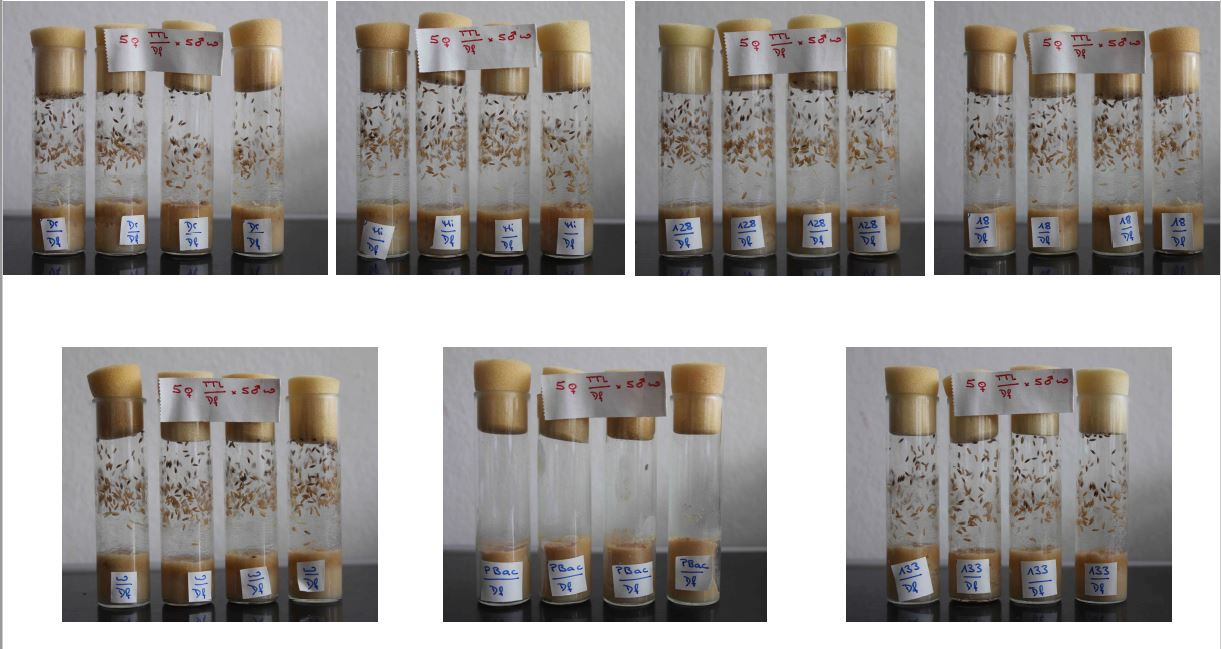
\includegraphics[width=1\linewidth]{img/fertility_test_results}
	\caption{}
	\label{fig:fertilitytestresults}
\end{figure}


% Please add the following required packages to your document preamble:
% \usepackage{graphicx}
\begin{table}[H]
	\centering
	\resizebox{\textwidth}{!}{%
		\begin{tabular}{|l|l|l|l|l|l|}
			\hline
			&  &  \begin{tabular}[c]{@{}l@{}}Hatching temp\\ of female\end{tabular} & Layed eggs & Unhatched eggs & Hatching rate \\ \hline
			4) &\T $w; \Tfrac{venus-TTLL}{venus-TTLL}; \Tfrac{venus-TTLL}{TM, Sb}$ \B & 25\degree C & 100 & 7 & 93 \\ \hline
			&\T  $w; \Tfrac{venus-TTLL}{Driver}; \Tfrac{venus-TTLL}{TM, Sb}$ \B & 25\degree C & 97 & 9 & 90.72 \\ \hline
			5) &\T  $w; \Tfrac{msps-mcherry}{msps-mcherry}$ \B & 25\degree C & 94 & 49 & 48 \\ \hline
			&\T  $w; \Tfrac{msps-mcherry}{TM, Sb}$ \B & 25\degree C & 100 & 48 & 52 \\ \hline
			&\T  $w;\Tfrac{Driver}{+} \Tfrac{msps-mcherry}{+}$ \B & 25\degree C & 100 & 67 & 33 \\ \hline
			&\T  $w;\Tfrac{Driver}{+} \Tfrac{msps-mcherry}{+}$ \B & 25\degree C & 9 & 4 & (56) \\ \hline
			6) &\T  $w;\Tfrac{TACC-mcherry}{TACC-mcherry}$ \B & 25\degree C & 91 & 29 & 68 \\ \hline
			&\T  $w;\Tfrac{TACC-mcherry}{TM, Sb}$ \B & 25\degree C & 88 & 66 & 25 \\ \hline
			&\T  $w; \Tfrac{Driver}{+}; \Tfrac{TACC-mcherry}{+}$ \B & 25\degree C & 111 & 79 & 29 \\ \hline
			2) &\T  $w; \Tfrac{venus-TTLL}{SM, Cy}; \Tfrac{Minos}{Df(TTLL)}$ \B & 29\degree C & 30 & 9 & 70 \\ \hline
			& \T $w; \Tfrac{venus-TTLL}{Driver}; \Tfrac{Minos}{Df(TTLL)}$ \B & 29\degree C & 73 & 6 & 92 \\ \hline
			4) &\T  $w; \Tfrac{venus-TTLL}{venus-TTLL}; \Tfrac{venus-TTLL}{TM, Sb}$ \B & 29\degree C & 86 & 17 & 80 \\ \hline
			&\T  $w; \Tfrac{venus-TTLL}{Driver}; \Tfrac{venus-TTLL}{TM, Sb}$ \B & 29\degree C & 85 & 14 & 84 \\ \hline
		\end{tabular}%
	}
\end{table}


%----------------------------------------------------------------------------------------
%	SECTION 3
%----------------------------------------------------------------------------------------
\newpage
\section*{Experiment 2: Confocal microscopy}



%----------------------------------------------------------------------------------------
%	SECTION 4
%----------------------------------------------------------------------------------------
\newpage
\section*{Experiment 3: Western blot}

%----------------------------------------------------------------------------------------
%	SECTION 5
%----------------------------------------------------------------------------------------
\newpage
\section*{Experiment 4: CRISPR/Cas9}


%----------------------------------------------------------------------------------------
%	SECTION 6
%----------------------------------------------------------------------------------------
\newpage
\section*{Conclusion and discussion}




%----------------------------------------------------------------------------------------
%	BIBLIOGRAPHY
%----------------------------------------------------------------------------------------

\bibliographystyle{apalike}

\bibliography{sample}

%----------------------------------------------------------------------------------------


\end{document}